\documentclass[onecolumn]{aastex62}


\newcommand{\vdag}{(v)^\dagger}
\newcommand\aastex{AAS\TeX}
\newcommand\latex{La\TeX}
\usepackage{listings}
\usepackage{amsmath}
\usepackage{physics}
\usepackage{hyperref}
\usepackage{natbib}
\usepackage[T1]{fontenc}
\usepackage[english]{babel}
\usepackage[utf8]{inputenc}

\begin{document}

\title{\Large Milestone I:\\Computing the Hubble parameter and conformal time.}





\author{Håkon Tansem}



\section{Introduction} \label{sec:intro}
Milestone I is the first part of a project consisting of four Milestones. The
main goal of the project is to calculate the CMB power spectrum. In
Milestone I, we will study the background evolution of the universe. To do this
we will compute the Hubble parameter from early times to today as
to describe the expansion history of the universe. We will also study the
evolution of the density parameters for baryons, cold dark matter, photons and
cosmological constant as well as the conformal time.
 
\section{Method} \label{sec:method}
When calculating the conformal time we start with the differential equation
\begin{equation}
    \frac{d\eta}{dt} = \frac{c}{a},
\end{equation}
where $\eta$ is the conformal time, $c$ is the speed of light, $a$ is the scale
factor and $t$ is time. By performing a change of variables by multiplying with
$\frac{dx}{dx}$ we get
\begin{equation}
    \frac{d\eta}{dx}\frac{dx}{dt} = \frac{c}{a},
\end{equation}
where we introduce the coordinate change $x=log(a)$. Using that
$\frac{dx}{dt}=H$ (\cite{callin2006calculate}), where $H$ is the hubble
paramater, we get an ODE we can solve for $\eta$ as
\begin{equation}\label{eq:eta_of_x}
    \frac{d\eta}{dx} = \frac{c}{\mathcal{H}(x)},
\end{equation}
where $\mathcal{H}(x)=e^xH(x)$ is the scaled Hubble parameter given in our new coordinate system. By neglecting density parameters for neutrinos
and curvature, we have and expression for the Hubble parameter given by
\begin{equation}\label{eq:H_of_x}
    H(x) = H_0\sqrt{(\Omega_{b,0} + \Omega_{CDM,0})e^{-3x} + \Omega_{r,0} e^{-4x} + \Omega_{\Lambda,0}}, \text{ (\cite{Winther:2020})}
\end{equation} 
where $H_0$ is the Hubble parameter today, $\Omega_{b,0}$ is the density parameter for baryons,
$\Omega_{CDM,0}$ is for cold dark matter, $\Omega_{r,0}$ is for radiation and
$\Omega_{\Lambda,0}$ is for cosmological constant. The sub index $0$ for the
density parameters represents
the value for the parameters today. The values for the density parameters today
are given as follows
\begin{align}
    \Omega_{CDM,0} &=0.25\\
    \Omega_{b,0} &=0.05\\
    \Omega_{\Lambda,0} &=0.7.
\end{align}
The parameter for radiation today is given as 
\begin{equation}
    \Omega_{r,0} =2\frac{\pi^2(k_bT_{cmb}^4)}{30\hbar^3c^5}\frac{8\pi G}{3H_0^2},
\end{equation}
where $G$ is the gravitational constant, $k_b$ is the Boltzmann constant and
$T_{cmb} =2.7255$K is the temperature of the CMB measured today (\cite{Winther:2020}).
 

We also want to study how the density parameters evolve with time. For the density parameters, we
have that 
\begin{align}
    \Omega_i &= \frac{\rho_i}{\rho_{c}} \\
             &= \frac{8\pi G}{3H(x)^2}\rho_i\\
             &= \frac{8\pi G}{3H(x)^2}\rho_{i,0}e^{-3x(1+w_i)},
\end{align}
where $\rho_{i,0}$ is the density today and $w$ is the equation of state parameter defined as $w_i\equiv\frac{P_i}{\rho_i}$, where $P_i$ is pressure and
$\rho_i$ is density for a given contribution to energy component $i$. By using the relation $\rho_{i,0} = \rho_{c,0}\Omega_{i,0}$, we get the
expression for a given density parameter as 
\begin{equation}
    \Omega_i(x)=\frac{H_0^2}{H(x)^2}e^{-3x(1+w_i)}\Omega_{i,0}.
\end{equation}
Using that $w_{CDM} = 0$, $w_{b} = 0$, $w_{\Lambda} = -1$ and $w_{r} = 1/3$
(\cite{Winther:2020}), we can now calculate the evolution of the density parameters for a given
$x$. We also want to study the evolution of the Hubble parameter as a function of redshift $z$. Using the relation $a(t) = \frac{1}{1+z}$,
we get, by substituting $a = e^x$, that the redshift as a function of our new
coordinate system is given as
\begin{equation}
    z = e^{-x} - 1.
\end{equation}

\section{Results/Discussion} \label{sec:results}
Figure (\ref{fig:densityparams}) shows the evolution of the density parameters
$\Omega$ as a function of $x=log(a)$. Here we can see that in early times the
universe was heavily dominated by radiation. At around $x=-8.0$ matter-radiation
equality occurs and at $x\approx-5.0$ the universe is matter dominated. At
around $x=0.0$ the universe starts to become dominated by a cosmological constant.

\begin{figure}
    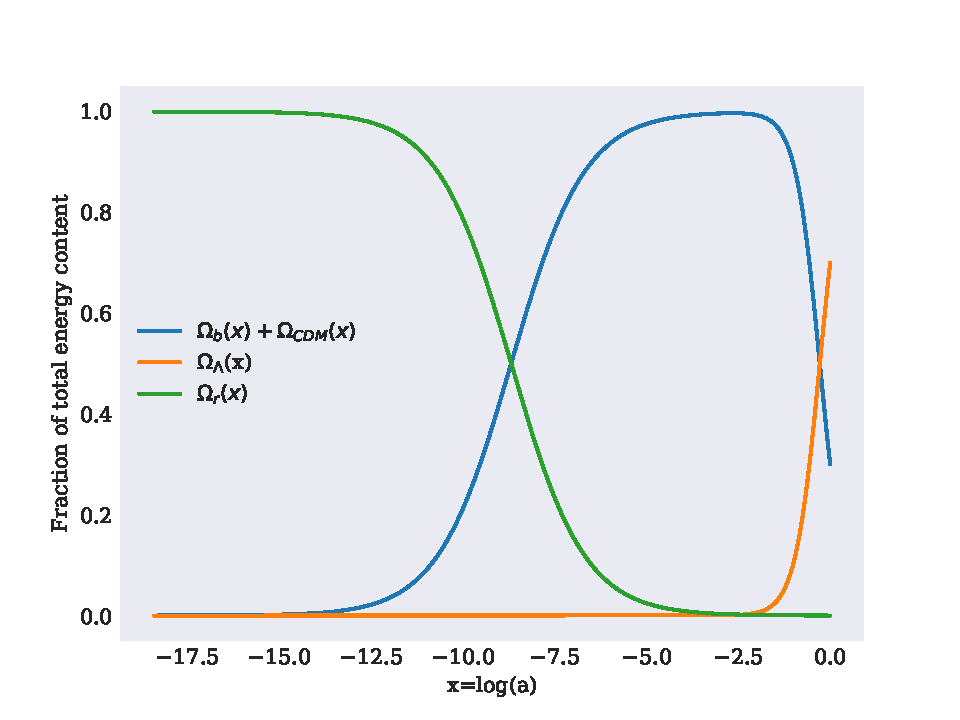
\includegraphics[scale=0.8]{figures/densityparams.pdf}
    \caption{Figure showing the evolution of the density parameters $\Omega$ for CDM, radiation and cosmological constant as a function of $x=log(a)$.}
    \label{fig:densityparams}
\end{figure}

Figure (\ref{fig:evolution}) shows the evolution of the conformal time, the
Hubble parameter and the scaled Hubble parameter as functions of $x$ as well as
the Hubble parameter as a function of redshift $z$. For early times we see that
the Hubble parameter is very large making the universe expand fast. As time goes
on the Hubble parameter decreases. By looking at the plot for the Hubble
parameter as a function of redshift $z$, we can see that by the time the CMB is
released, at $z\approx1100$, the Hubble parameter has decreased by a factor of
around $10^7\sim10^8$. This shows that the early universe expanded very fast
before it slowed down during the onset of matter domination. From the
plots for $H(x)$ and $\mathcal{H}(x)$, we can also see a slight change in slope
which coincides with the same value for $x$ as matter-radiation equality in
Figure \ref{fig:densityparams}. One can also see, while studying the plot for
the conformal time $\eta$, that it is almost inversely proportional to the
expansion rate. When the expansion rate is at its highest, the horizon grows the
fastest. From the scaled Hubble parameter, which can be interpreted as
$\dot{a}$, we can see that the expansion is decelerating throughout the
radiation dominated and matter dominated eras. The expansion rate seems to
accelerate again when the universe enters cosmological constant dominated era at
around $x=0$, which is indicated by $\mathcal{H}(x)$ gaining a positive slope,
but the equations were not solved going into the future. 

\begin{figure}
    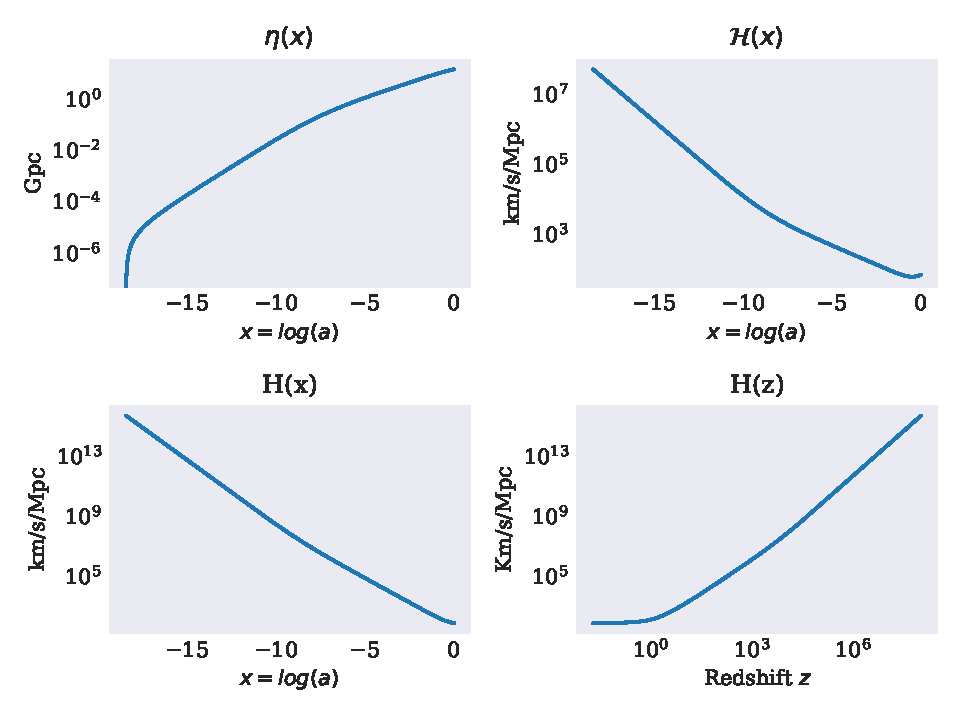
\includegraphics[scale=0.8]{figures/evolution.pdf}
    \caption{Starting clockwise from the top left, the figure shows the evolution of the conformal time $\eta$ as a function of $x$, the scaled Hubble parameter as a function of $x$, the hubble paramater as a function of redshift $z$ and the Hubble parameter as a function of $x$.}
    \label{fig:evolution}
\end{figure}
\section{Benchmark}
The time elapsed for calculating eta turned out to be 0.000474332 sec measured
using the C++ chrono library.


\bibliography{ref.bib}
\bibliographystyle{aasjournal}
%\begin{thebibliography}{}
%\end{thebibliography}
\end{document}

% End of file `sample62.tex'.
